% (find-LATEX "2020-1-C2-fracs-parcs.tex")
% (defun c () (interactive) (find-LATEXsh "lualatex -record 2020-1-C2-fracs-parcs.tex" :end))
% (defun D () (interactive) (find-pdf-page      "~/LATEX/2020-1-C2-fracs-parcs.pdf"))
% (defun d () (interactive) (find-pdftools-page "~/LATEX/2020-1-C2-fracs-parcs.pdf"))
% (defun e () (interactive) (find-LATEX "2020-1-C2-fracs-parcs.tex"))
% (defun u () (interactive) (find-latex-upload-links "2020-1-C2-fracs-parcs"))
% (defun v () (interactive) (find-2a '(e) '(d)) (g))
% (find-pdf-page   "~/LATEX/2020-1-C2-fracs-parcs.pdf")
% (find-sh0 "cp -v  ~/LATEX/2020-1-C2-fracs-parcs.pdf /tmp/")
% (find-sh0 "cp -v  ~/LATEX/2020-1-C2-fracs-parcs.pdf /tmp/pen/")
%   file:///home/edrx/LATEX/2020-1-C2-fracs-parcs.pdf
%               file:///tmp/2020-1-C2-fracs-parcs.pdf
%           file:///tmp/pen/2020-1-C2-fracs-parcs.pdf
% http://angg.twu.net/LATEX/2020-1-C2-fracs-parcs.pdf
% (find-LATEX "2019.mk")
% (find-C2-aula-links "2020-1-C2-fracs-parcs" "16" "fracparc")

% «.video»		(to "video")
%
% «.defs»		(to "defs")
% «.title»		(to "title")
% «.2020_deriv_ln.mp4»	(to "2020_deriv_ln.mp4")
% «.exercicio-4»	(to "exercicio-4")
% «.djvuize»		(to "djvuize")


% «video»  (to ".video")
% (find-ssr-links     "c2m201divcomresto" "2020_div_com_resto")
% (code-eevvideo      "c2m201divcomresto" "2020_div_com_resto")
% (code-eevlinksvideo "c2m201divcomresto" "2020_div_com_resto")
% (find-c2m201divcomrestovideo "0:00")

\documentclass[oneside,12pt]{article}
\usepackage[colorlinks,citecolor=DarkRed,urlcolor=DarkRed]{hyperref} % (find-es "tex" "hyperref")
\usepackage{amsmath}
\usepackage{amsfonts}
\usepackage{amssymb}
\usepackage{pict2e}
\usepackage[x11names,svgnames]{xcolor} % (find-es "tex" "xcolor")
%\usepackage{colorweb}                 % (find-es "tex" "colorweb")
%\usepackage{tikz}
%
% (find-dn6 "preamble6.lua" "preamble0")
%\usepackage{proof}   % For derivation trees ("%:" lines)
%\input diagxy        % For 2D diagrams ("%D" lines)
%\xyoption{curve}     % For the ".curve=" feature in 2D diagrams
%
\usepackage{edrx15}               % (find-LATEX "edrx15.sty")
\input edrxaccents.tex            % (find-LATEX "edrxaccents.tex")
\input edrxchars.tex              % (find-LATEX "edrxchars.tex")
\input edrxheadfoot.tex           % (find-LATEX "edrxheadfoot.tex")
\input edrxgac2.tex               % (find-LATEX "edrxgac2.tex")
%
%\usepackage[backend=biber,
%   style=alphabetic]{biblatex}            % (find-es "tex" "biber")
%\addbibresource{catsem-slides.bib}        % (find-LATEX "catsem-slides.bib")
%
% (find-es "tex" "geometry")
\usepackage[a6paper, landscape,
            top=1.5cm, bottom=.25cm, left=1cm, right=1cm, includefoot
           ]{geometry}
%
\begin{document}

\catcode`\^^J=10
\directlua{dofile "dednat6load.lua"}  % (find-LATEX "dednat6load.lua")

% %L dofile "edrxtikz.lua"  -- (find-LATEX "edrxtikz.lua")
% %L dofile "edrxpict.lua"  -- (find-LATEX "edrxpict.lua")
% \pu

% «defs»  (to ".defs")
% (find-LATEX "edrx15.sty" "colors-2019")
\long\def\ColorRed   #1{{\color{Red1}#1}}
\long\def\ColorViolet#1{{\color{MagentaVioletLight}#1}}
\long\def\ColorViolet#1{{\color{Violet!50!black}#1}}
\long\def\ColorGreen #1{{\color{SpringDarkHard}#1}}
\long\def\ColorGreen #1{{\color{SpringGreenDark}#1}}
\long\def\ColorGreen #1{{\color{SpringGreen4}#1}}
\long\def\ColorGray  #1{{\color{GrayLight}#1}}
\long\def\ColorGray  #1{{\color{black!30!white}#1}}
\long\def\ColorBrown #1{{\color{Brown}#1}}
\long\def\ColorBrown #1{{\color{brown}#1}}

\long\def\ColorShort #1{{\color{SpringGreen4}#1}}
\long\def\ColorLong  #1{{\color{Red1}#1}}

\def\frown{\ensuremath{{=}{(}}}
\def\True {\mathbf{V}}
\def\False{\mathbf{F}}
\def\D    {\displaystyle}

\def\drafturl{http://angg.twu.net/LATEX/2020-1-C2.pdf}
\def\drafturl{http://angg.twu.net/2020.1-C2.html}
\def\draftfooter{\tiny \href{\drafturl}{\jobname{}} \ColorBrown{\shorttoday{} \hours}}

% (find-angg ".emacs" "c2q192")


%  _____ _ _   _                               
% |_   _(_) |_| | ___   _ __   __ _  __ _  ___ 
%   | | | | __| |/ _ \ | '_ \ / _` |/ _` |/ _ \
%   | | | | |_| |  __/ | |_) | (_| | (_| |  __/
%   |_| |_|\__|_|\___| | .__/ \__,_|\__, |\___|
%                      |_|          |___/      
%
% «title»  (to ".title")
% (c2m201fracparcp 1 "title")
% (c2m201fracparc    "title")

\thispagestyle{empty}

\begin{center}

\vspace*{1.2cm}

{\bf \Large Cálculo 2 - 2020.1}

\bsk

Aulas 16 e 17: Frações parciais

\bsk

Eduardo Ochs - RCN/PURO/UFF

\url{http://angg.twu.net/2020.1-C2.html}

\end{center}

\newpage

% «2020_deriv_ln.mp4»  (to ".2020_deriv_ln.mp4")
% (c2m201fracparcp 2 "2020_deriv_ln.mp4")
% (c2m201fracparc    "2020_deriv_ln.mp4")
% (find-twusfile "eev-videos/")
% (find-twusfile "eev-videos/" "2020_deriv_ln.mp4")
% (find-eevvideo-links "derivln" "2020_deriv_ln" "0:00")
% (code-video "derivlnvideo" "$S/http/angg.twu.net/eev-videos/2020_deriv_ln.mp4")
% (find-derivlnvideo "0:00")
% (find-derivlnvideo "2:48" "aparece em C1 mas ninguém dá muita bola pra ela")
% (find-derivlnvideo "4:15" "pode ser calculada de dois jeitos diferentes")
% (find-derivlnvideo "4:41" "f'(g(x))g'(x) = 1")
% (find-derivlnvideo "5:52" "[DFI]")
% (find-derivlnvideo "7:44" "[DFI][substs] = (...)")
% (find-derivlnvideo "8:30" "d/dx ln x = 1/x")
% (find-derivlnvideo "8:48" "ln x = \\int 1/x dx")
% (find-derivlnvideo "9:11" "num primeiro momento a gente não sabe se isso é verdade")

Neste vídeo nós vimos que $\frac{d}{dx} \ln x = 1/x$...

\ssk

\url{http://angg.twu.net/eev-videos/2020_deriv_ln.mp4}

\ssk

e aí começamos a fazer exercícios de integração...

\bsk

{\bf Exercício 1.}

% (find-fline "~/LATEX/2020-1-C2/20201112_C2_fracoes_parciais_1.pdf")
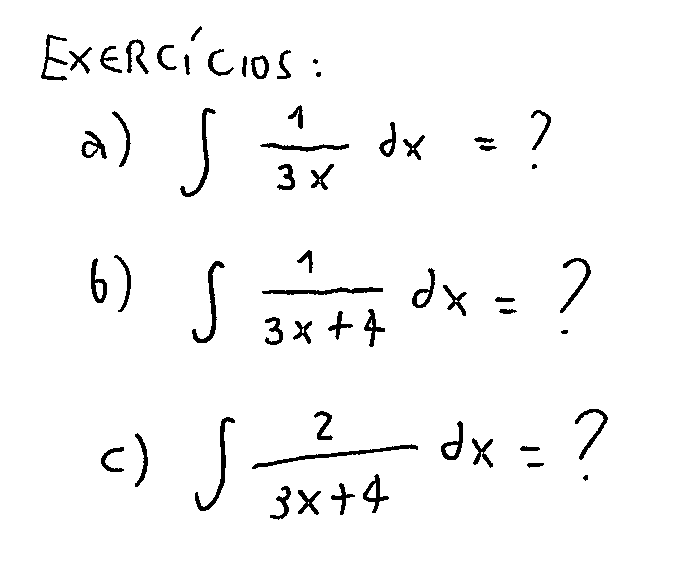
\includegraphics[height=5cm]{2020-1-C2/20201112_C2_fracoes_parciais_1.pdf}

\newpage

% (find-fline "~/LATEX/2020-1-C2/20201112_C2_fracoes_parciais_2.pdf")
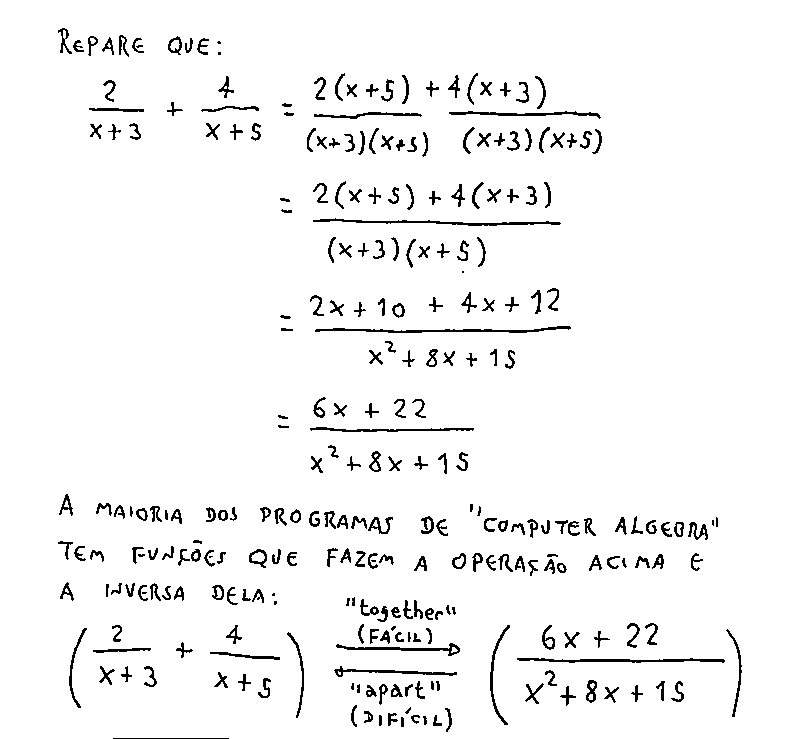
\includegraphics[height=8cm]{2020-1-C2/20201112_C2_fracoes_parciais_2.pdf}

\newpage

{\bf Exercício 2.}

% (find-fline "~/LATEX/2020-1-C2/20201112_C2_fracoes_parciais_3.pdf")
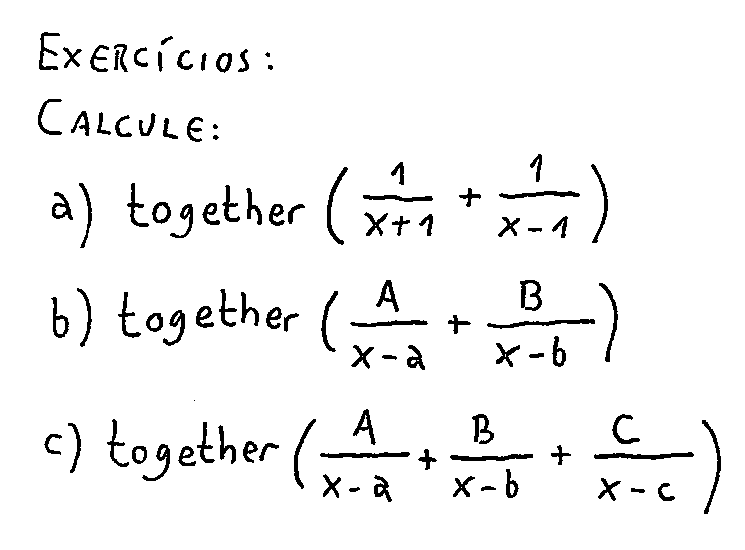
\includegraphics[height=7cm]{2020-1-C2/20201112_C2_fracoes_parciais_3.pdf}

\newpage

{\bf Exercício 3.}

% (find-fline "~/LATEX/2020-1-C2/20201112_C2_fracoes_parciais_4.pdf")
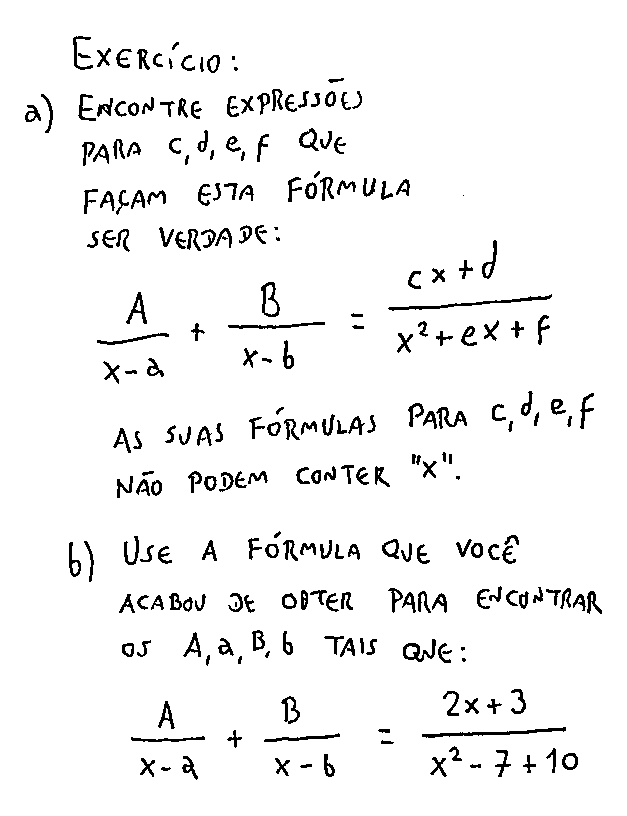
\includegraphics[height=7cm]{2020-1-C2/20201112_C2_fracoes_parciais_4.pdf}

\newpage

{\bf Slogan: contas sem ``vai um'' podem ser traduzidas

pra contas com polinômios.}

\ssk

O que mais nos interessa pra Frações Parciais

é \ColorRed{divisão com resto}. Exemplo:

% (find-fline "~/LATEX/2020-1-C2/20201118_C2_div_com_resto_1.pdf")
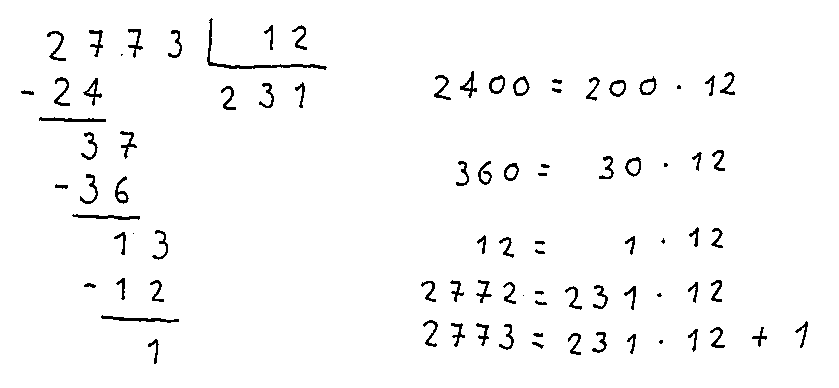
\includegraphics[width=11cm]{2020-1-C2/20201118_C2_div_com_resto_1.pdf}

\newpage

...e tradução do exemplo para polinômios:

% (find-fline "~/LATEX/2020-1-C2/20201118_C2_div_com_resto_2.pdf")
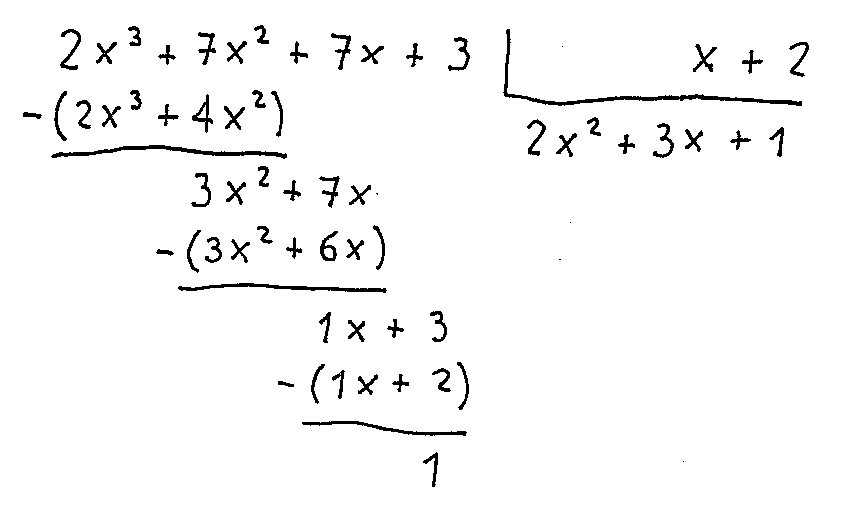
\includegraphics[height=4cm]{2020-1-C2/20201118_C2_div_com_resto_2.pdf}

% (find-fline "~/LATEX/2020-1-C2/20201118_C2_div_com_resto_3.pdf")
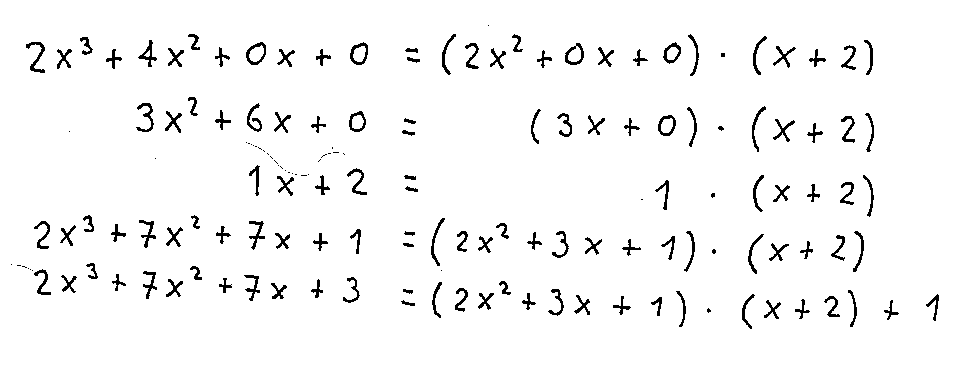
\includegraphics[height=3cm]{2020-1-C2/20201118_C2_div_com_resto_3.pdf}

\newpage

% «exercicio-4»  (to ".exercicio-4")
% (c2m201fracparcp 99 "exercicio-4")
% (c2m201fracparc     "exercicio-4")

{\bf Exercício 4.}

\ssk

Use estas idéias para integrar:

$$\intx{\frac{2x^3 + 7x^2 + 7x + 3}{x+2}} \;\; = \;\; ?$$



\newpage

{\bf Exercício 5.}

\ssk

O que acontece nos casos em que ``teria vai um''?

\ssk

a) Tente fazer a divisão com resto de $x^3$ por $x+2$.

Mais precisamente, encontre um polinômios $R(x)$ e $Q(x)$ tais que

$(x^3) = Q(x) · (x+2) + R(x)$ e $R(x)$ é no máximo de grau 1.

Teste a sua resposta!

\ssk

b) Calcule $\intx{\frac{x^3}{x+2}}$ pelo método acima.

Teste a sua resposta derivando a sua antiderivada para $\frac{x^3}{x+2}$.

\ssk

c) Calcule $\intx{\frac{x^3}{x+2}}$ fazendo a substituição $u=x+2$.

Você deve obter o mesmo resultado que na (b).

\bsk

d) Calcule $\intx{\frac{x^2}{(x+1)(x-1)}}$ por frações parciais.


\newpage

{\bf Dica importante}

\ssk

Lembre que uns dos meus slogans é

``eu só vou corrigir os sinais de igual''...

No slide 7 a igualdade mais importante é a da última linha.

Nós vamos usá-la assim, pra transformar a integral original

em algo fácil de integrar:

\msk

% (find-fline "~/LATEX/2020-1-C2/20201119_C2_div_com_resto_4.pdf")
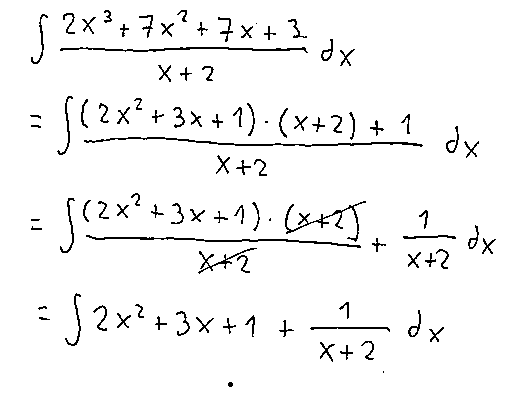
\includegraphics[height=4cm]{2020-1-C2/20201119_C2_div_com_resto_4.pdf}







\end{document}

%  ____  _             _         
% |  _ \(_)_   ___   _(_)_______ 
% | | | | \ \ / / | | | |_  / _ \
% | |_| | |\ V /| |_| | |/ /  __/
% |____// | \_/  \__,_|_/___\___|
%     |__/                       
%
% «djvuize»  (to ".djvuize")

 (eepitch-shell)
 (eepitch-kill)
 (eepitch-shell)
# (find-fline "~/2020.1-C2/")
# (find-fline "~/LATEX/2020-1-C2/")
# (find-fline "~/bin/djvuize")

cd ~/2020.1-C2/
rm -v  20201112_C2_fracoes_parciais*.png
rm -v  20201112_C2_fracoes_parciais*.pdf

f () { djvuize WHITEBOARDOPTS="-m 0.5" $* } 
f 20201112_C2_fracoes_parciais_1.pdf
f 20201112_C2_fracoes_parciais_2.pdf
f 20201112_C2_fracoes_parciais_3.pdf
f 20201112_C2_fracoes_parciais_4.pdf

cd ~/2020.1-C2/
f () { djvuize WHITEBOARDOPTS="-m 0.5" $* } 
rm -v 20201118_C2_div_com_resto*.png
rm -v 20201118_C2_div_com_resto*.pdf
f 20201118_C2_div_com_resto_1.pdf
f 20201118_C2_div_com_resto_2.pdf
f 20201118_C2_div_com_resto_3.pdf

f 20201119_C2_div_com_resto_4.pdf


 (eepitch-shell)
 (eepitch-kill)
 (eepitch-shell)
cp -v  ~/LATEX/2020-1-C2-fracs-parcs.pdf /tmp/
cd /tmp/
xournalpp 2020-1-C2-fracs-parcs.pdf

%  __  __       _        
% |  \/  | __ _| | _____ 
% | |\/| |/ _` | |/ / _ \
% | |  | | (_| |   <  __/
% |_|  |_|\__,_|_|\_\___|
%                        
% <make>

 (eepitch-shell)
 (eepitch-kill)
 (eepitch-shell)
# (find-LATEXfile "2019planar-has-1.mk")
make -f 2019.mk STEM=2020-1-C2-fracs-parcs veryclean
make -f 2019.mk STEM=2020-1-C2-fracs-parcs pdf

% Local Variables:
% coding: utf-8-unix
% ee-tla: "c2m201fracparc"
% End:
